\documentclass[journal]{IEEEtran}
\usepackage[T1]{fontenc}
\usepackage[utf8]{inputenc}
\usepackage{amsmath,amssymb}
\usepackage{booktabs,array,multirow}
\usepackage{microtype}
\usepackage{url}
\usepackage{cite}
\usepackage{algorithm}
\usepackage{algpseudocode}
\usepackage{listings}
\usepackage{tikz}
\usetikzlibrary{arrows.meta,positioning,fit}
\usepackage[hidelinks]{hyperref}

\lstset{basicstyle=\ttfamily\footnotesize,breaklines=true,columns=fullflexible,
  frame=single,framerule=0.3pt,xleftmargin=2pt,xrightmargin=2pt,aboveskip=4pt,belowskip=4pt,
  keepspaces=true,literate={−}{-}1}
\newcommand{\code}[1]{\texttt{#1}}
\newcommand{\SynodSQL}{SynodSQL}
\newcolumntype{L}[1]{>{\raggedright\arraybackslash}p{#1}}
\renewcommand{\arraystretch}{1.1}

\hyphenation{Synod-SQL check-points tomb-stones}

\begin{document}
\title{\SynodSQL: A Git-Style Replication Model for Fully Replicated, Trusted Peer Databases}
\author{Jean-Luc~Robitaille%
\thanks{J.-L. Robitaille is an independent author (e-mail: jlr@robitaille.us).}}
\markboth{Draft, October 2026}{Robitaille: \SynodSQL}
\maketitle

\begin{abstract}
This paper describes \SynodSQL, a replication model for a small network of trusted servers. Every server holds a full copy of all data and writes locally at all times. At fixed intervals (epochs), all servers merge their changes into one shared state. The merge is an $N$-way git-style merge with one common base: the state at the end of the previous epoch. The merge function is deterministic, so every server computes the same result without a central merge step. A Merkle root hash of the result lets the servers prove that they agree. The paper gives the storage layout, the sync protocol, the merge algorithm, a taxonomy of write conflicts with a rule for each type, a worked example, and a model of the conflict rate. Conflicts that rules cannot resolve become rows in a replicated conflict table. They never stop the merge. The model gives up global serializability. In exchange, it gives local writes with no network wait, full offline operation, and simple recovery.
\end{abstract}

\begin{IEEEkeywords}
Replicated databases, eventual consistency, deterministic merge, conflict resolution, Merkle trees, version control.
\end{IEEEkeywords}

\section{Motivation}
\IEEEPARstart{E}{arly} ARPANET design had one clear goal: resource sharing among a set of known, trusted hosts \cite{roberts1970}. The hosts belonged to research institutions that trusted each other. Shared data, such as the host table HOSTS.TXT, was copied to every site \cite{harrenstien1985}.

HOSTS.TXT had one writer. Every other host only read it. This design failed as the network grew, because the single writer became a bottleneck. DNS then split ownership into zones.

This paper asks a different question: what if every trusted host can write, and every host keeps all data? Each host then works at local speed, and it continues to work when the network is down. The cost is that hosts must merge their changes, and concurrent changes can conflict.

Version control systems solved a similar problem for source code. Git lets many people change copies of the same files and merge them later. This paper applies the git model to database rows, with three changes:
\begin{enumerate}
\item The merge runs automatically on a fixed schedule, not by hand.
\item Every host computes the merge itself, and all hosts get the same result.
\item A conflict does not block the merge. It becomes data that people or programs resolve later.
\end{enumerate}

\section{Assumptions and Scope}
The model assumes a small, closed group of trusted nodes that hold all data. Section~\ref{sec:limits} discusses what fails when an assumption is false. Table~\ref{tab:assume} lists the assumptions.

\begin{table*}[t]
\caption{Assumptions and Their Consequences}\label{tab:assume}
\centering\small
\begin{tabular}{@{}L{2.8cm}L{6.8cm}L{7.4cm}@{}}
\toprule
Assumption & Meaning & Consequence\\
\midrule
Trusted nodes & No node lies or attacks. Nodes can still crash, have bugs, or lose disks. & No signatures or Byzantine fault tolerance. Checksums are still necessary.\\
Closed membership & A known set of $N$ nodes. Peers authenticate with a shared secret or mutual TLS. & Outsiders cannot join or inject data.\\
Full replication & Every node stores all data. & Storage per node equals the full database size.\\
Small $N$ & Tens of nodes, up to low hundreds. & All-to-all exchange per epoch is acceptable.\\
Periodic sync & The merge runs once per epoch (minutes to one day). & Other nodes see a write after at most one epoch plus sync time.\\
Local-first writes & A write commits locally with no network wait. & No global serializability.\\
Loosely synced clocks & Clocks drift. Hybrid logical clocks (HLC) \cite{kulkarni2014} limit the effect. & Tie-breaks are deterministic and close to real-time order.\\
\bottomrule
\end{tabular}
\end{table*}

Out of scope are open networks, untrusted peers, partial replication, and workloads that need strict global invariants at every instant (Section~\ref{sec:invariants}).

\section{Storage Model}\label{sec:storage}
Each node stores the database in one file, similar to SQLite. Only row content is shared between nodes. Everything else in the file is local and derived, so each node can rebuild it at any time.

\subsection{Heap Pages}
Table rows live in unordered heap pages. Each row has a header and column values:
\begin{lstlisting}
row_id     128-bit logical ID:
           node ID (32) + counter (64) + reserved (32)
stamp[c]   per-column HLC time + node ID of
           the last write to column c
flags      live | tombstone
values[c]  column values
\end{lstlisting}
The row ID never changes. Two nodes cannot make the same ID, so a merge never renumbers rows. The per-column stamps let the merge compare a late write with the newest write to that column (Section~\ref{sec:late}).

\subsection{Row Map}
A B-tree maps \code{row\_id} to \code{(page, slot)}. It is local, because physical addresses are different on each node.

\subsection{Secondary Indexes}
B-trees map column values to \code{row\_id}. They are local and derived. After each merge, a node updates them for the changed rows, or bulk-loads them again. A rebuild is also a chance to apply an access-weighted layout that puts frequently read keys near the root.

\subsection{State Hash Tree}
A Prolly tree (a content-defined Merkle B-tree, as in Dolt \cite{dolt}) maps \code{row\_id} to the hash of the row content. Its node boundaries come from content hashes, so the same data always gives the same tree, whatever the order of inserts. The root hash therefore identifies the full shared state. Two nodes with the same root hash hold the same data. Two nodes with different hashes can find the differing rows by a walk down the differing subtrees only.

\subsection{Epoch Log}
During an epoch, every local write also goes to an epoch log. Each entry holds the row ID, the operation, the transaction ID, the HLC time, the before-image, and the after-image. The log is the node's branch for this epoch. Its size is proportional to the rows that the node changed, not to the database size. The before-images also keep the epoch base readable, so the node does not need a second copy of the database.

\section{The Epoch Model}
Time is divided into epochs. Every epoch starts from the same shared state on every node and ends with one $N$-way merge. Each node writes to its own epoch log. At the end of the epoch, every node runs the same merge on the same inputs and gets the same root hash (Fig.~\ref{fig:epoch}).

\begin{figure}[t]
\centering
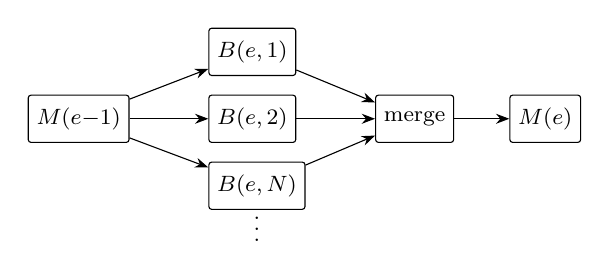
\begin{tikzpicture}[font=\footnotesize,>=Stealth,
  box/.style={draw,rounded corners=1pt,align=center,minimum height=0.6cm,inner sep=3pt},
  node distance=0.45cm and 0.5cm]
\node[box] (m0) {$M(e{-}1)$};
\node[box,right=1.0cm of m0,yshift=0.85cm] (b1) {$B(e,1)$};
\node[box,right=1.0cm of m0] (b2) {$B(e,2)$};
\node[box,right=1.0cm of m0,yshift=-0.85cm] (b3) {$B(e,N)$};
\node[box,right=1.0cm of b2] (mg) {merge};
\node[box,right=0.7cm of mg] (m1) {$M(e)$};
\draw[->] (m0) -- (b1); \draw[->] (m0) -- (b2); \draw[->] (m0) -- (b3);
\draw[->] (b1) -- (mg); \draw[->] (b2) -- (mg); \draw[->] (b3) -- (mg);
\draw[->] (mg) -- (m1);
\node[below=0.05cm of b3,yshift=0.3cm,xshift=0.0cm] {$\vdots$};
\end{tikzpicture}
\caption{One epoch. Every node starts from the same base $M(e{-}1)$, writes to its own log $B(e,i)$, and then runs the same deterministic merge.}\label{fig:epoch}
\end{figure}

The terms are:
\begin{itemize}
\item $M(e{-}1)$: the merged state at the start of epoch $e$. All nodes hold an identical copy.
\item $B(e,i)$: the epoch log of node $i$ in epoch $e$, which holds its changes against $M(e{-}1)$.
\item $M(e)=\mathrm{merge}\bigl(M(e{-}1);B(e,1),\dots,B(e,N)\bigr)$: the merged state at the end of epoch $e$.
\end{itemize}

The key simplification is that every log in epoch $e$ has the same merge base, $M(e{-}1)$. Git must search a commit graph to find a merge base. Here the base is always known, so the merge is a simple three-way comparison for each row.

\subsection{The Git Analogy}
Table~\ref{tab:git} maps git concepts to \SynodSQL. Two differences matter. First, in git one person makes a merge commit and pushes it. Here every node computes the merge, and the root hash proves that all nodes agree. Second, a git conflict stops the merge until a person fixes it. Here a conflict never stops the merge.

\begin{table}[t]
\caption{Git Concepts and Their \SynodSQL{} Counterparts}\label{tab:git}
\centering\small
\begin{tabular}{@{}L{3.5cm}L{4.6cm}@{}}
\toprule
Git & \SynodSQL\\
\midrule
Repository & Database file on one node\\
Commit & Local transaction\\
Branch & A node's epoch log $B(e,i)$\\
Merge base & Previous merged state $M(e{-}1)$\\
Octopus merge & The $N$-way epoch merge\\
Merge driver & Column merge policy in the schema\\
Conflict markers & Rows in the \code{\_conflicts} table\\
Rebase & Late and in-flight writes applied on top of the new $M(e)$\\
Revert & A revert log in a later epoch\\
Clone & Full copy for a node more than $L$ epochs behind\\
Tree hash & Prolly tree root hash\\
\bottomrule
\end{tabular}
\end{table}

\section{Sync Protocol}\label{sec:sync}
Each epoch has a write phase and a sync phase. The sync phase has five steps, and only step~3 needs any coordination.
\begin{enumerate}
\item \emph{Seal.} At the epoch boundary (by HLC time), each node closes its epoch log $B(e,i)$. New local writes go to the next log, $B(e{+}1,i)$. The node computes a hash of the sealed log.
\item \emph{Exchange.} Each node sends its sealed log to the other nodes. For small $N$, every node sends to every other node. For larger $N$, nodes use gossip: each node forwards the logs it has to a few random peers in each round. Gossip reaches all nodes in about $\log_2 N$ rounds \cite{demers1987}.
\item \emph{Agree on the manifest.} All nodes must merge the same set of logs, or they compute different states. The epoch leader (node $e \bmod N$, or the next node in order if that node is down) publishes a manifest: the list of log hashes in epoch $e$. A log that does not arrive before the deadline goes into a later epoch (Section~\ref{sec:late}).
\item \emph{Merge.} Each node runs the deterministic merge (Section~\ref{sec:merge}) on $M(e{-}1)$ and the logs in the manifest. The result is $M(e)$, the conflict rows for epoch $e$, and the root hash $H(e)$.
\item \emph{Verify and switch.} Nodes exchange $H(e)$. If the hashes match, each node makes $M(e)$ its new base, re-applies its in-flight writes from $B(e{+}1,i)$ on top of $M(e)$, and updates its local indexes. A node with a different hash has a bug or bad data. It fetches the differing subtrees of $M(e)$ from a peer and raises an alert.
\end{enumerate}

\emph{In-flight writes.} Writes made during the sync phase are in $B(e{+}1,i)$. Each entry keeps its own before-image and HLC time. The next merge treats them by the same rules as late writes (Section~\ref{sec:late}), so no special rebase logic is necessary.

\emph{Split leaders.} During a network split, two nodes can each act as leader and publish different manifests. Nodes accept the manifest from the highest-priority leader they can reach. If a node later sees a higher-priority manifest for the same epoch, it discards its $M(e)$ and merges again. This is safe, because $M(e)$ is derived data and no log is lost. For strict agreement, the manifest can go through a consensus log such as Raft \cite{ongaro2014}. A manifest is only a list of hashes, so the cost is low.

\emph{Traffic.} With all-to-all exchange, total traffic per epoch is about $N(N-1)\Delta$, where $\Delta$ is the mean log size. With gossip or relays, each node sends about $\Delta\times$fanout. Every node already holds $M(e{-}1)$, so no node sends the full database in normal operation.

\section{The Merge Algorithm}\label{sec:merge}
The merge is a pure function of $M(e{-}1)$ and the logs in the manifest. It does not depend on which node runs it, on arrival order, or on local clocks. This gives the main property of the model: all nodes that use the same manifest get the same $M(e)$.

\subsection{Per-Row Merge}
For each row that at least one log changed:
\begin{enumerate}
\item Collect the changes from all logs and sort them by node ID. If one node changed the row more than once, keep only its last after-image, with its first before-image.
\item If only one node changed the row, take its after-image.
\item If more than one node changed the row:
 \begin{enumerate}
 \item If any change is a delete, apply the delete rule (Section~\ref{sec:delete}).
 \item Else, merge column by column. A node changed a column if its after-image differs from its before-image.
  \begin{itemize}
  \item No node changed the column: keep the current value.
  \item All changing nodes wrote the same value: take that value.
  \item Nodes wrote different values: apply the column policy (Section~\ref{sec:policies}).
  \end{itemize}
 \end{enumerate}
\end{enumerate}
Row IDs are unique, so two nodes never insert the same row. An insert always enters step~2.

\subsection{Constraint Pass}
After all rows merge, the merge checks unique keys, foreign keys, and check constraints on $M(e)$. Each violation becomes a constraint conflict (Sections~\ref{sec:unique}--\ref{sec:invariants}). The fix for each violation must also be deterministic.

\subsection{Pseudocode}
Algorithm~\ref{alg:merge} gives the merge.

\begin{algorithm}[t]
\caption{Deterministic epoch merge}\label{alg:merge}
\small
\begin{algorithmic}[1]
\Function{Merge}{$base$, $logs$} \Comment{$logs$ sorted by node ID}
 \State $changes \gets$ group all log entries by \texttt{row\_id}
 \State $result \gets$ \Call{CopyOnWrite}{$base$}; $conflicts \gets [\,]$
 \For{\textbf{each} $r$ \textbf{in} sorted($changes$)}
  \State $cs \gets changes[r]$
  \If{$|cs|=1$}
   \State \Call{Apply}{$result, cs[0]$}
  \ElsIf{any $c\in cs$ is a delete}
   \State \Call{ResolveDelete}{$result, r, cs, conflicts$}
  \Else
   \State $row \gets$ copy of $result[r]$
   \For{\textbf{each} column $col$}
    \State $W \gets \{c\in cs : c.after[col]\neq c.before[col]\}$
    \If{$W=\emptyset$} \textbf{continue} \EndIf
    \If{all $c.after[col]$ equal for $c\in W$}
     \State $row[col]\gets W[0].after[col]$
    \Else
     \State $row[col]\gets$ \Call{Resolve}{$col, row[col], W, conflicts$}
    \EndIf
   \EndFor
   \State $result.put(r,row)$
  \EndIf
 \EndFor
 \State \Call{CheckConstraints}{$result, conflicts$} \Comment{unique, FK, check}
 \State sort $conflicts$ by (table, row ID, column)
 \State \Return $result$, $conflicts$, \Call{RootHash}{$result$}
\EndFunction
\end{algorithmic}
\end{algorithm}

\section{Conflict Taxonomy and Resolution}\label{sec:taxonomy}
Most concurrent writes merge automatically. Only unique keys, foreign keys, and cross-row invariants need a person. Table~\ref{tab:taxonomy} lists every conflict type the model can produce, from common and easy to rare and hard.

\begin{table*}[t]
\caption{Conflict Types and Default Rules}\label{tab:taxonomy}
\centering\small
\begin{tabular}{@{}l L{3.2cm} L{4.6cm} L{3.4cm} L{2.6cm}@{}}
\toprule
Sec. & Type & Example & Default rule & Needs a person?\\
\midrule
\ref{sec:nonconf} & Disjoint rows & A changes row 1, B changes row 2 & Take both & No\\
\ref{sec:nonconf} & Same row, different columns & A changes price, B changes name & Take both columns & No\\
\ref{sec:policies} & Same column, different values & A sets price 0.12, B sets 0.11 & Column policy & Only with a flag policy\\
\ref{sec:delete} & Update and delete & A deletes a row, B updates it & Delete wins, B's version recorded & Optional\\
\ref{sec:unique} & Unique key collision & A and B each insert a part with SKU C-400 & Earliest insert keeps the key & Yes\\
\ref{sec:fk} & Orphan foreign key & A inserts an order for customer 7, B deletes customer 7 & Undo the delete, record it & Yes\\
\ref{sec:invariants} & Broken invariant & Stock is 5, A sells 4, B sells 3 & Keep result and record it, or prevent with escrow & Yes, or design it out\\
\ref{sec:schema} & Schema change & A adds a column, B renames it & Not allowed in normal epochs & Not applicable\\
\bottomrule
\end{tabular}
\end{table*}

\subsection{No-Conflict Cases}\label{sec:nonconf}
Most concurrent writes touch different rows or different columns. A column-level merge removes a large class of false conflicts that a row-level merge would report. Git works at line level for the same reason: two edits to different lines of one file merge cleanly.

\subsection{Same Column, Different Values: Column Policies}\label{sec:policies}
Each column declares a merge policy in the schema, like a git merge driver in \code{.gitattributes}:
\begin{lstlisting}
CREATE TABLE inventory (
  row_id  ROWID,
  sku     TEXT UNIQUE              MERGE lww,
  name    TEXT                     MERGE lww,
  price   DECIMAL(10,2)            MERGE lww_flag,
  qty     INTEGER CHECK (qty >= 0) MERGE delta,
  tags    SET<TEXT>                MERGE union,
  notes   TEXT                     MERGE text3
);
\end{lstlisting}
Table~\ref{tab:policies} lists the policies.

\begin{table}[t]
\caption{Column Merge Policies}\label{tab:policies}
\centering\footnotesize
\begin{tabular}{@{}l L{2.9cm} L{1.5cm} L{1.8cm}@{}}
\toprule
Policy & Rule & Good for & Risk\\
\midrule
\code{lww} & Highest (HLC, node ID) wins & Names, status & Other write lost silently\\
\code{lww\_flag} & As \code{lww}; losing values go to \code{\_conflicts} & Prices, settings & Review work\\
\code{delta} & current $+\sum(\text{after}-\text{before})$ over all writers & Counters, balances & Can break a check (Sec.~\ref{sec:invariants})\\
\code{max}, \code{min} & Largest or smallest value & High-water marks & Cannot lower (raise) the value\\
\code{union} & (current $\cup$ additions) $-$ removals & Tags, member lists & A removal wins over a keep\\
\code{text3} & Line-level three-way text merge, in node ID order & Notes, long text & Overlaps become conflicts\\
\code{flag} & Keep current value, record all values & Data that must not change silently & Most review work\\
\bottomrule
\end{tabular}
\end{table}

The \code{delta} policy matters most. With \code{lww}, a sale on node A and a sale on node B produce a lost update: one sale disappears. With \code{delta}, both sales count. This is the same idea as a PN-counter CRDT \cite{shapiro2011}. The common base also makes \code{union} clean: within one epoch, a node can only remove items that were in the base, and it can only add items that were not, so an add and a remove of the same item cannot both occur.

\subsection{Update and Delete}\label{sec:delete}
Node A deletes a row. Node B updates the same row in the same epoch. Each table selects one of three rules:
\begin{itemize}
\item \emph{Delete wins} (default). The row becomes a tombstone. B's after-image goes to \code{\_conflicts}.
\item \emph{Update wins.} The row stays, with B's values. A's delete goes to \code{\_conflicts}.
\item \emph{Flag.} The row stays as a tombstone with B's values attached, and a person decides.
\end{itemize}
Delete wins is the default because a delete is usually deliberate. The record in \code{\_conflicts} means that no data is lost.

\subsection{Unique Key Collision}\label{sec:unique}
Row IDs never collide, but user values can. Node A and node B each insert a part with SKU C-400. The merged table now has two rows with one unique value, and the merge cannot know which row is right.

\emph{Rule:} the row whose insert has the earliest (HLC, node ID) keeps the value. The other row moves to \code{\_conflicts}, with a reference to the winner. A person or program then merges the two rows, renames one, or discards one.

\emph{Prevention:} use generated keys where possible. Where users must choose keys, give each node a key range or prefix. For example, only node A makes SKUs that start with \code{A-}.

\subsection{Orphan Foreign Key}\label{sec:fk}
Node A inserts an order for customer 7. Node B deletes customer 7. Each change is valid on its own node, but together they break the foreign key.

\emph{Rule:} undo the delete of the parent row (restore it from $M(e{-}1)$), and record a conflict that names both changes. This loses no data. A table can select cascade delete instead.

\subsection{Invariants Across Rows or Values}\label{sec:invariants}
Some rules cannot survive a merge. Stock is 5. Node A sells 4, and node B sells 3. Each sale is valid locally, because each node saw 5 in stock. The delta merge gives $5-4-3=-2$, which breaks $\texttt{qty}\ge 0$.

No merge rule can fix this after the fact, because the goods are already sold twice. Bailis et al.\ call the needed property \emph{invariant confluence} (I-confluence): an invariant is safe under merge only if a merge of two valid states always gives a valid state \cite{bailis2014}. Table~\ref{tab:iconf} gives examples.

\begin{table}[t]
\caption{Invariants and Merge Safety}\label{tab:iconf}
\centering\small
\begin{tabular}{@{}L{5.6cm}l@{}}
\toprule
Invariant & Safe under merge?\\
\midrule
Unique generated ID & Yes\\
Unique user-chosen value & No\\
Foreign key, inserts only & Yes\\
Foreign key, with deletes & No\\
$\texttt{qty}\ge 0$, increments only & Yes\\
$\texttt{qty}\ge 0$, with decrements & No\\
\texttt{start} $<$ \texttt{end}, columns changed on different nodes & No\\
\bottomrule
\end{tabular}
\end{table}

For an unsafe invariant, a table selects one of three approaches:
\begin{itemize}
\item \emph{Accept and repair.} Keep the merged result and record a conflict. A person or program repairs it later, for example with a backorder or a refund. Many real businesses already work this way.
\item \emph{Escrow.} Split the resource between nodes before the epoch. With stock 5 and two nodes, A may sell up to 3 and B up to 2. Each node checks its own share locally. The merge then gives out new shares by a fixed rule, for example in equal parts. The invariant holds with no coordination during the epoch.
\item \emph{Coordinate.} Send that one operation to a single owner node or a consensus group. This gives up local writes for that operation only.
\end{itemize}

\subsection{Schema Changes}\label{sec:schema}
Two nodes that change the schema in different ways produce data that cannot merge. So schema changes do not go through normal epochs. A schema change is a special manifest entry. All nodes must acknowledge it before the epoch that applies it. In that epoch, the merge first migrates $M(e{-}1)$ and every log entry with the same migration function, and then merges as usual.

\subsection{The \texttt{\_conflicts} Table}
Each recorded conflict becomes one row:
\begin{lstlisting}
_conflicts(
  conflict_id  hash of (epoch, table, row_id,
               column, kind); same on all nodes
  epoch, table, row_id, column, kind,
  base_value,
  values       list of (node_id, hlc, value)
  applied_value, rule,
  status       open | resolved
)
\end{lstlisting}
The \code{\_conflicts} table is a normal replicated table. Any node can resolve a conflict: it writes the chosen value to the data row and sets \code{status} to \code{resolved}. The resolution travels in the next epoch like any other write. If two nodes resolve the same conflict differently in one epoch, the result is a new same-column conflict, which \code{lww\_flag} handles. In practice this ends quickly, because it needs two people to act on the same conflict in the same epoch.

\section{Worked Example}
In one epoch, three nodes make nine writes to an inventory table. The merge completes with no stop and records three conflicts for review. The table uses the policies from Section~\ref{sec:policies} (\code{name} lww, \code{price} lww\_flag, \code{qty} delta, \code{sku} unique) and the delete-wins rule.

Table~\ref{tab:base} shows the base state $M(e{-}1)$, and Table~\ref{tab:writes} shows the writes during epoch $e$.

\begin{table}[t]
\caption{Base State $M(e{-}1)$}\label{tab:base}
\centering\small
\begin{tabular}{@{}llllr@{}}
\toprule
row\_id & sku & name & price (USD) & qty\\
\midrule
r1 & A-100 & Bolt, M6 & 0.10 & 500\\
r2 & A-200 & Nut, M6 & 0.05 & 800\\
r3 & B-310 & Washer, M6 & 0.02 & 1000\\
\bottomrule
\end{tabular}
\end{table}

\begin{table}[t]
\caption{Writes During Epoch $e$}\label{tab:writes}
\centering\small
\begin{tabular}{@{}cc l L{4.6cm}@{}}
\toprule
Node & HLC & Row & Change\\
\midrule
A & 10 & r1 & price 0.10 $\to$ 0.12\\
B & 11 & r1 & name $\to$ Bolt, M6 x 20\\
A & 12 & r2 & qty 800 $\to$ 650 (sold 150)\\
B & 13 & r2 & qty 800 $\to$ 700 (sold 100)\\
A & 14 & r3 & delete\\
B & 15 & r3 & qty 1000 $\to$ 900\\
B & 16 & r4 (new) & insert C-400, Spacer, 0.08, qty 200\\
C & 17 & r1 & price 0.10 $\to$ 0.11\\
C & 18 & r5 (new) & insert C-400, Spacer 10 mm, 0.09, qty 50\\
\bottomrule
\end{tabular}
\end{table}

The merge goes row by row:
\begin{itemize}
\item \textbf{r1.} Only B changed \code{name}, so the merge takes it. A and C changed \code{price} to different values. Policy \code{lww\_flag}: C has the later HLC (17 against 10), so price becomes 0.11. A's value 0.12 goes to \code{\_conflicts}.
\item \textbf{r2.} A and B both changed \code{qty}. Policy \code{delta}: $800+(650-800)+(700-800)=550$. Both sales count, with no conflict. With \code{lww}, the result would be 700, and A's sale of 150 would disappear.
\item \textbf{r3.} A deleted the row, and B updated it. Delete wins. B's after-image (qty 900) goes to \code{\_conflicts}.
\item \textbf{r4, r5.} The row IDs are different, so the per-row pass takes both. The constraint pass then finds two rows with SKU C-400. B's insert has the earlier HLC (16 against 18), so r4 keeps the key. r5 moves to \code{\_conflicts}.
\end{itemize}

\begin{table}[t]
\caption{Result $M(e)$}\label{tab:result}
\centering\small
\begin{tabular}{@{}llllr@{}}
\toprule
row\_id & sku & name & price (USD) & qty\\
\midrule
r1 & A-100 & Bolt, M6 x 20 & 0.11 & 500\\
r2 & A-200 & Nut, M6 & 0.05 & 550\\
r4 & C-400 & Spacer & 0.08 & 200\\
\bottomrule
\end{tabular}
\end{table}

\begin{table}[t]
\caption{\texttt{\_conflicts} for Epoch $e$}\label{tab:wconf}
\centering\footnotesize
\begin{tabular}{@{}l L{1.5cm} L{1.7cm} L{1.7cm} L{1.2cm}@{}}
\toprule
Target & Kind & Applied & Recorded & Rule\\
\midrule
r1.price & Same column & 0.11 (C) & 0.12 (A) & lww\_flag\\
r3 & Update and delete & Deleted (A) & qty 900 (B) & Delete wins\\
r5 & Unique key C-400 & r4 keeps C-400 (B) & r5, Spacer 10 mm (C) & Earliest insert\\
\bottomrule
\end{tabular}
\end{table}

Tables~\ref{tab:result} and~\ref{tab:wconf} show the outcome. All three nodes compute these exact tables and the same root hash $H(e)$. A person now reviews three conflicts. The other changes, including both concurrent sales on r2, needed no review.

\section{Conflict Rate Analysis}
Conflicts per unit time grow linearly with epoch length and with the square of the node count, so shorter epochs and small groups keep review work low.

\emph{Model.} Take $N$ nodes. In one epoch, each node writes $w$ rows. Each write goes to row $i$ with probability $p_i$. A row conflicts if two or more nodes write it in the same epoch. When $w p_i$ is small, the chance that one node writes row $i$ is about $w p_i$, and the expected number of conflicting rows per epoch is
\begin{equation}
\mathbb{E}[\text{conflicting rows}] \approx \binom{N}{2} w^2 \sum_i p_i^2 .
\end{equation}
For uniform access over $R$ rows, $\sum_i p_i^2 = 1/R$. With a write rate of $r$ per node and an epoch length of $T$, $w=rT$. Conflicts per unit time are then
\begin{equation}
\frac{\mathbb{E}[\text{conflicting rows}]}{T} \approx \frac{N(N-1)\,r^2\,T}{2R}.
\end{equation}
The results are:
\begin{itemize}
\item The conflict rate grows linearly with epoch length $T$. Halving $T$ halves the conflicts per day.
\item It grows with $N^2$, so the model suits small groups.
\item Skew dominates. The sum $\sum_i p_i^2$ is the collision probability of the access pattern. If 1\% of all writes go to one row, that one row alone adds $10^{-4}$, the same as uniform access over only 10{,}000 rows.
\end{itemize}

\emph{Example.} Take $N=5$ nodes, $r=1{,}000$ writes per hour per node, $R=1{,}000{,}000$ rows, and uniform access (Table~\ref{tab:rate}). These are row-level conflicts. Column-level merge and mergeable policies (\code{delta}, \code{max}, \code{union}) resolve most of them with no record. Only flag-type policies and constraint conflicts reach a person.

\begin{table}[t]
\caption{Expected Conflicting Rows for the Example}\label{tab:rate}
\centering\small
\begin{tabular}{@{}lrrr@{}}
\toprule
Epoch length & $w$ per node & Rows/epoch & Rows/day\\
\midrule
1 day & 24{,}000 & $\approx$5{,}760 & $\approx$5{,}760\\
1 hour & 1{,}000 & $\approx$10 & $\approx$240\\
5 minutes & 83 & $\approx$0.07 & $\approx$20\\
\bottomrule
\end{tabular}
\end{table}

\emph{Design rules.} (i) Make hot columns mergeable: use \code{delta}, \code{max}, or \code{union} on columns that many nodes write. (ii) Choose the epoch length from the acceptable conflict rate, not only from bandwidth. (iii) Keep user-chosen unique keys out of hot paths, because those conflicts always need review.

\section{Correctness and Consistency Properties}
The model guarantees convergence and bounded staleness. It does not guarantee global serializability.

\emph{Guaranteed:}
\begin{itemize}
\item \emph{Convergence.} Two nodes that apply the same sequence of manifests reach the same state. Proof sketch: $M(0)$ is the same on all nodes. Each $M(e)$ is a deterministic function of $M(e{-}1)$ and the logs in manifest $e$. The manifest names logs by hash, so all nodes use the same inputs. By induction, all $M(e)$ are equal. The root hash check in step~5 detects any break in this chain, such as a bug or a bad disk.
\item \emph{Local durability.} A write is durable on its node when the local transaction commits.
\item \emph{Bounded staleness.} A write in manifest $e$ is visible on all live nodes after the sync of epoch $e$. The bound is one epoch plus sync time.
\item \emph{Read your writes.} A node always sees its own writes, also before the merge.
\item \emph{Local isolation.} Transactions on one node are serializable with respect to that node's view, as in SQLite.
\item \emph{No lost updates on mergeable columns.} The \code{delta}, \code{max}, \code{min}, and \code{union} policies keep the effect of every write.
\end{itemize}

\emph{Not guaranteed:}
\begin{itemize}
\item \emph{Global serializability.} Two nodes can each run a transaction that is valid locally, and the merged result may not equal any serial order. Write skew is possible, and so are lost updates on \code{lww} columns.
\item \emph{Invariants that are not I-confluent} (Section~\ref{sec:invariants}). The model detects and records each break, but it does not prevent it.
\item \emph{Atomic transactions across the merge.} Conflict rules apply per row. A transaction that changed rows r1 and r2 can win on r1 and lose on r2. A group of tables can opt in to transaction-level resolution: if any row of a transaction loses, all rows of that transaction go to \code{\_conflicts}. The transaction ID in each log entry makes this possible, and it stays deterministic.
\end{itemize}
In CAP terms, the model chooses availability. Every node accepts reads and writes during a network partition. Consistency is eventual, with a bound of one epoch while the network is up.

\section{Failures, Late Nodes, and Garbage Collection}
Missing logs wait for a later epoch, nodes that fall too far behind clone a peer, and tombstones stay until no older log can arrive.

\subsection{A Node Misses the Deadline}\label{sec:late}
Node $k$ is offline at the end of epoch $e$, so its log $B(e,k)$ is not in manifest $e$. The other nodes merge without it. When node $k$ comes back, it fetches the current state from a peer. The Prolly tree diff sends only the subtrees that changed. Node $k$ then submits $B(e,k)$, which goes into the next manifest as a late log.

The merge handles a late log with the normal rules, because each log entry carries its own before-image and HLC time:
\begin{itemize}
\item \code{delta} adds the entry's own change (after $-$ before) to the current value. The late sale still counts.
\item \code{lww} compares the entry's HLC with the column stamp in the current state. An old write loses to any newer write, which is the correct result.
\item A column counts as changed if the entry's after-image differs from its own before-image, not from the current value.
\end{itemize}
In-flight writes from the sync phase (Section~\ref{sec:sync}) use the same mechanism.

\emph{Lateness bound $L$.} A node that is more than $L$ epochs behind cannot submit its old logs as normal writes, because the tombstones they depend on may be gone (Section~\ref{sec:gc}). It clones the current state of a peer. Its old log entries go to \code{\_conflicts} as stale writes for review.

\subsection{Crash During the Merge}
The merge writes $M(e)$ beside $M(e{-}1)$ by copy-on-write. The switch is one atomic pointer update in the file header. After a crash before the switch, the node still has $M(e{-}1)$ and the logs, so it runs the merge again. The result is the same, because the merge is deterministic.

\subsection{Tombstones and Garbage Collection}\label{sec:gc}
A deleted row stays as a tombstone, so that a late write cannot bring it back. The Xerox Clearinghouse used the same idea and called the records death certificates \cite{demers1987}. A tombstone from epoch $e$ can be removed after epoch $e+L$, because no log older than $L$ epochs is accepted. The same bound lets nodes drop old logs, old manifests, and resolved \code{\_conflicts} rows.

\subsection{Leader Failure}
If the epoch leader is down, the next node in order publishes the manifest after a timeout. Section~\ref{sec:sync} describes the rule for two leaders during a network split.

\subsection{A Node with a Bug}
A bug in the merge on one node gives a different root hash, and step~5 detects it. A bug that writes bad data into a log is harder, because the log is valid input. All logs and manifests stay available for $L$ epochs, so the nodes can undo the damage with a revert log in a later epoch, like \code{git revert}.

\section{Related Work}
Most parts of this model exist in earlier systems. The contribution is the combination: one common merge base per epoch, a deterministic merge on every node, and conflicts as replicated rows that never block the merge. Table~\ref{tab:related} compares the closest systems.

\begin{table*}[t]
\caption{Related Systems}\label{tab:related}
\centering\small
\begin{tabular}{@{}L{4.0cm}L{6.6cm}L{6.4cm}@{}}
\toprule
System & What it shares with this model & Main difference\\
\midrule
Xerox Clearinghouse, epidemic algorithms \cite{demers1987} & Fully replicated database on trusted servers; anti-entropy; death certificates & Last-writer-wins only; no conflict records\\
Bayou \cite{terry1995} & Weakly connected replicas; merge procedures per application; dependency checks & A primary server fixes the final order; writes stay tentative until then\\
Lotus Notes & Replication between trusted servers; conflict documents kept for review & Document level, not column level\\
CouchDB & Every replica picks the same winning revision; losing revisions kept as conflicts & Document level; no common base per epoch\\
Git \cite{chacon2014} & Branches, three-way merge, merge drivers, rebase, revert & Merges by hand; a conflict blocks the merge\\
Dolt \cite{dolt} & SQL with git-style branches, cell-level three-way merge, conflict tables, Prolly trees & Merges are explicit user actions, not automatic merges among peers\\
cr-sqlite and CRDTs \cite{shapiro2011,crsqlite} & Merge without coordination; per-column last-writer-wins and counters & No conflicts are recorded; every merge is silent\\
Calvin \cite{thomson2012} & Replicas stay identical because they run deterministic logic on agreed input & Agrees on input order before execution, so writes wait for the network\\
Invariant confluence \cite{bailis2014} & Theory of which invariants survive a merge & Theory, not a system\\
\bottomrule
\end{tabular}
\end{table*}

The closest single system is Dolt. \SynodSQL{} is roughly Dolt with an automatic, scheduled octopus merge among peers, where every node computes the merge and the root hash proves agreement.

\section{Limitations and Open Questions}\label{sec:limits}
The model fits a small group of trusted nodes with mostly mergeable data, and it fits badly where those assumptions fail.

\emph{Limitations:}
\begin{itemize}
\item \emph{Storage.} Every node holds the full database, so total storage is $N$ times the data size.
\item \emph{Scale.} Traffic and conflicts grow with $N^2$. Above a few hundred nodes, use relays or partition the data.
\item \emph{Contended invariants.} Bank balances, seat bookings, and stock with hard limits need escrow or coordination (Section~\ref{sec:invariants}). The model detects the problem but does not remove it.
\item \emph{Staleness.} Other nodes see a write only after the merge. Some workflows cannot accept this.
\item \emph{Review load.} \code{lww\_flag}, \code{flag}, unique-key, and foreign-key conflicts need people. A busy system with long epochs can make thousands per day (Table~\ref{tab:rate}).
\item \emph{Trust.} One node with a bug can write bad data to all nodes. A revert repairs the data, but a person must first see the problem.
\item \emph{Clock dependence.} The \code{lww} order follows HLC time. Within the HLC drift bound, a node with a fast clock wins more contests.
\end{itemize}

\emph{Open questions:}
\begin{itemize}
\item What epoch length is best for a given write rate, bandwidth, and review budget? The conflict rate analysis gives a starting point.
\item Can the leader and manifest step go away? One option: include every log sealed before an HLC deadline, and merge again when a late log arrives.
\item Can transaction-level conflict resolution stay cheap for large transactions?
\item How well do automatic escrow rules work on real inventory data?
\item Does an access-weighted index layout, rebuilt at each merge, give a measurable read gain over a plain B-tree?
\end{itemize}

\section{Prototype and Evaluation Plan}
Nothing in this paper is measured yet. A prototype on SQLite can test every main claim. The merge layer can be a Python or Rust library on top of SQLite. The prototype parts are:
\begin{itemize}
\item Logical row IDs and per-column HLC stamps, as extra columns on each SQLite table.
\item An epoch log, filled by triggers that copy the before-image and after-image of every write.
\item A Prolly tree over (row ID, row hash) for the root hash and for catch-up diffs.
\item The merge function, with the policies in Section~\ref{sec:policies} and a \code{\_conflicts} table.
\item Sync over HTTP with mutual TLS, and a fixed leader rotation for manifests.
\end{itemize}
Table~\ref{tab:exp} lists the experiments.

\begin{table*}[t]
\caption{Planned Experiments}\label{tab:exp}
\centering\small
\begin{tabular}{@{}L{3.4cm}L{8.2cm}L{5.4cm}@{}}
\toprule
Claim & Experiment & Metric\\
\midrule
Convergence & 5 to 50 nodes, random writes, random crashes and late nodes, 10{,}000 epochs & Root hash mismatches (target: 0)\\
Determinism & Property-based test: random concurrent histories, random arrival order on each node & Identical $M(e)$ on every node\\
Conflict model & Uniform and Zipf workloads; vary $N$, $T$, and skew & Measured against predicted conflicting rows\\
Merge cost & Vary total log size $\Delta$ and database size $n$ & Merge time; check that it follows $\Delta$, not $n$\\
Sync cost & Vary $N$, fanout, and $\Delta$ & Bytes sent per node per epoch\\
Value of column policies & Same workload with \code{lww} only, then with all policies & Lost updates; conflicts that need review\\
Index rebuild & Plain B-tree against an access-weighted layout, rebuilt at each merge & Read latency at p50 and p99\\
\bottomrule
\end{tabular}
\end{table*}

\section{Conclusion}
A small network of trusted servers can share one database with full copies, local writes, and no central server. The key idea is a global epoch: all nodes merge from the same base with the same deterministic rules, so they reach the same state without a merge coordinator. Column policies resolve most concurrent writes automatically. The rest become rows in a replicated conflict table, and they never block work. The model gives up global serializability and invariants that are not I-confluent. In exchange, it gives the ARPANET goal of shared resources among trusted peers, with the merge discipline of git.

\bibliographystyle{IEEEtran}
\bibliography{references}

\end{document}
